%!TEX root = ../problems.tex
\begin{figure}[h!]
	\centering
	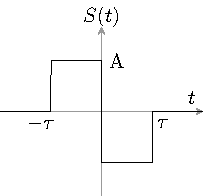
\includegraphics[width=0.4\linewidth]{ris/task15_input}
	\caption{Входное напряжение}
	\label{fig:15.1}
\end{figure}

\begin{task}
	Найти спектр сигнала, изображенного на рисунке. Нарисовать график $\abs{S(\omega)}$
\end{task}

\begin{proof}[\rm{\textbf{Решение}}]
	Зададим функцию с рисунка, а затем продифференцируем её:
	$$S(t)=A[\H(t+\tau)-\H(t)]+A[\H(t-\tau)-\H(t)]$$
	$$S'(t)=A[\delta(t+\tau)-\delta(t)]+A[\delta(t- \tau)-\delta(t)] $$
	По свойствам преобразования Фурье:
	\begin{equation}
		S'(\omega)=i \omega S(\omega) \Longrightarrow S(\omega)
		=\frac{S'(w)}{i \omega}
	\end{equation}
	Запишем преобразование Фурье:
	\begin{gather*}
		S'(\omega)=\newint S'(t)\cdot e^{-i \omega t} \dd{t}=
		A \newint \delta(t+ \tau) e^{-i \omega t} \dd{t}+
		A \newint \delta(t- \tau) e^{-i \omega t} \dd{t}+\\
		A \newint -2\delta(t) e^{-i \omega t} \dd{t}=
		A \qty(e^{+ i \omega \tau}+e^{-i \omega \tau}-2 )
	\end{gather*}
	Тогда:
	\begin{gather*}
		S(\omega)=\frac{A}{i \omega}
		\qty(e^{+ i \omega \tau}+e^{-i \omega \tau}-2 )=
		\frac{2A}{i \omega}(\cos{\omega \tau}-1)=
		\\
		\frac{2iA}{\omega}(1-\cos{\omega \tau})
	\end{gather*}
	\begin{equation}
		\abs{S(\omega)}=2A\abs{ \frac{1-\cos(\omega \tau)}{\omega} }
	\end{equation}
\begin{figure}[h!]
	\centering
	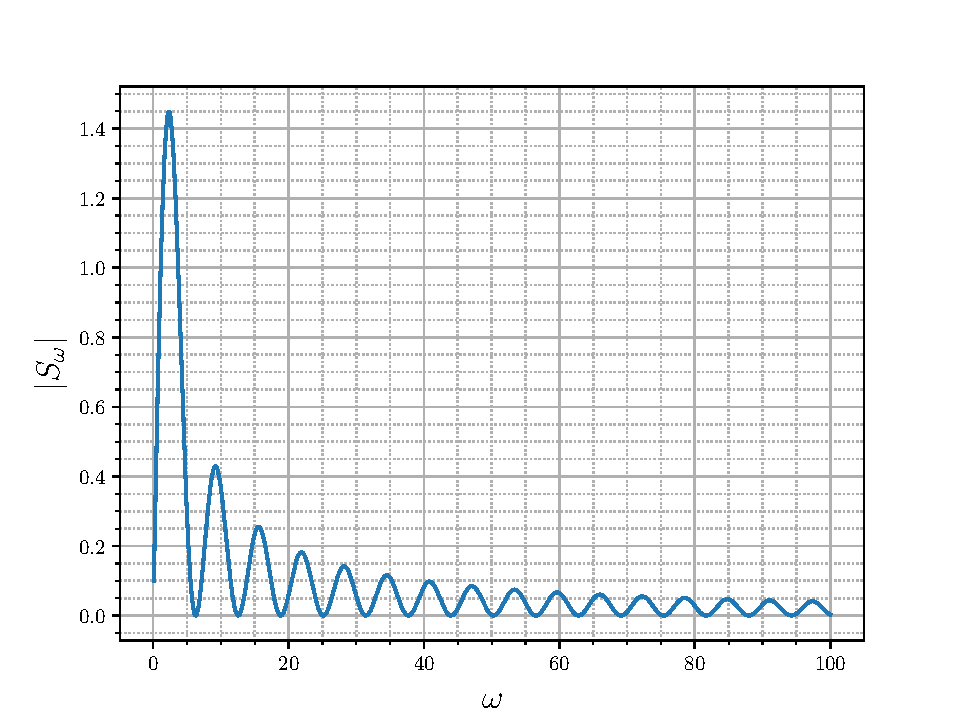
\includegraphics[width=0.7\linewidth]{ris/task15_out}
	\caption{Решение при $A=1,\tau=1$}
	\label{fig:15.2}
\end{figure}

\end{proof}

